\documentclass{beamer}
\setbeamertemplate{navigation symbols}{}

\usepackage{beamerthemeshadow}
\usepackage{amsmath}
\begin{document}
\title{Attractor dynamics and generalization bounds of rate-distortion networks trained via spike-timing dependent plasticity}  
\author{Clayton Seitz}
\date{\today} 

\begin{frame}[plain]
\titlepage
\end{frame}

\begin{frame}[plain]\frametitle{Table of contents}\tableofcontents
\end{frame} 

\section{Introduction} 

\begin{frame}[plain]
\frametitle{Introduction} 

\end{frame}

\begin{frame}[plain]
\frametitle{Training low-rate critical networks on uniform stimulus} 

\begin{equation*}
p_{ee} = 0.16 \; p_{ie} = 0.318 \;  p_{ei} = 0.244 \; p_{ii} = 0.343
\end{equation*}

\begin{equation*}
\mathcal{L}_{1} = \alpha \sum_{j} (r_{j} - \hat{r})^{2}
\end{equation*}

\begin{center}
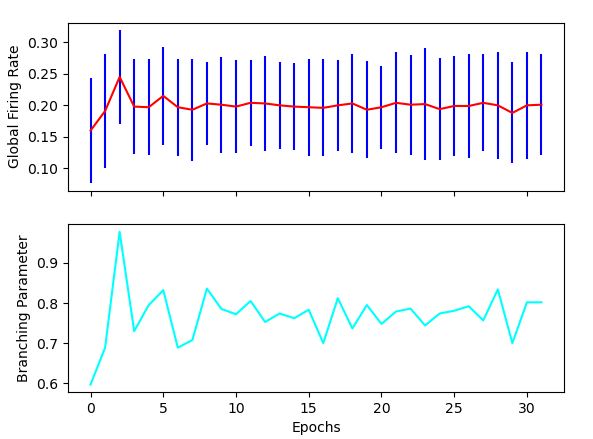
\includegraphics[scale=0.5]{sse-vars}
\end{center}

Training on an SSE of average rate per neuron (current setup)

\end{frame}


\begin{frame}[plain]
\frametitle{Training low-rate critical networks on uniform stimulus} 

\begin{equation*}
p_{ee} = 0.16 \; p_{ie} = 0.318 \;  p_{ei} = 0.244 \; p_{ii} = 0.343
\end{equation*}
\begin{equation*}
\mathcal{L}_{2} = \alpha\sum_{t} (r(t) - \hat{r})^{2}
\end{equation*}

\begin{center}
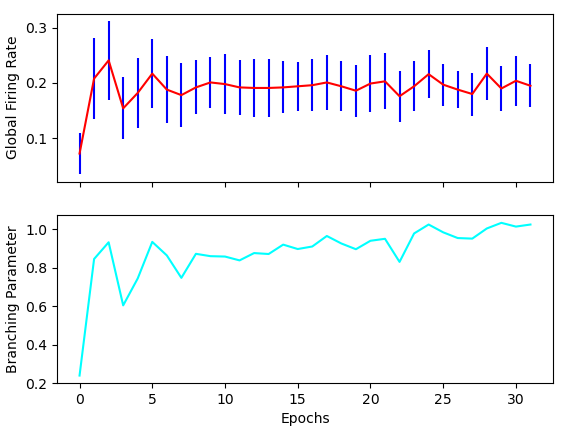
\includegraphics[scale=0.5]{alpha-1ms-bin}
\end{center}

Training on the instantaneous firing rate $r(t)$ reduces variability, improves branching parameter

\end{frame}

\begin{frame}[plain]
\frametitle{Training low-rate critical networks on uniform stimulus} 

\begin{equation*}
\mathcal{L}_{2} = \alpha\sum_{t} (r(t) - \hat{r})^{2}
\end{equation*}

\begin{center}
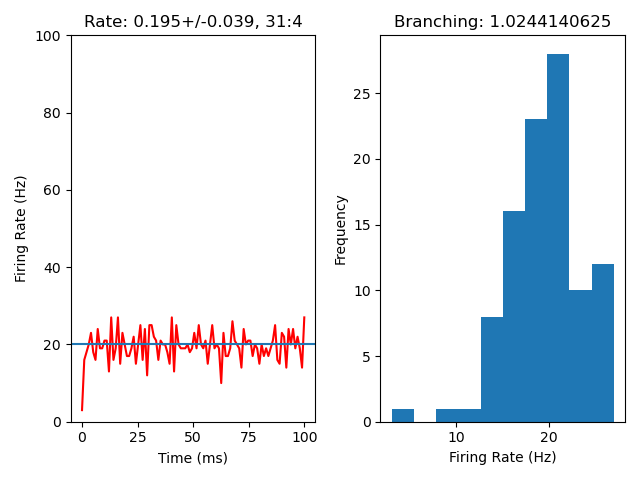
\includegraphics[scale=0.5]{last-epoch}
\end{center}


\end{frame}

\begin{frame}[plain]
\frametitle{} 

But optimization of $\mathcal{L}_{2}$ shows a more sparse response

\begin{center}
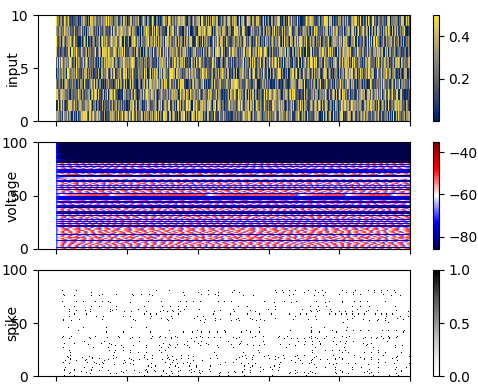
\includegraphics[scale=0.7]{alpha-traces}
\end{center}

\end{frame}

\begin{frame}[plain]
\frametitle{} 

Optimization of $\mathcal{L}_{1}$ doesn't

\begin{center}
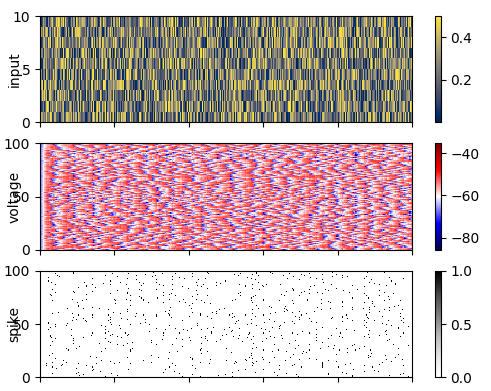
\includegraphics[scale=0.65]{global-traces}
\end{center}

\end{frame}


\begin{frame}[plain]
\frametitle{Balancing internal and recurrent inputs} 

We know something about the balance of excitation and inhibition that gives critical dynamics. What about the balance between input and recurrence? (Cramer et al. 2020)


\begin{center}
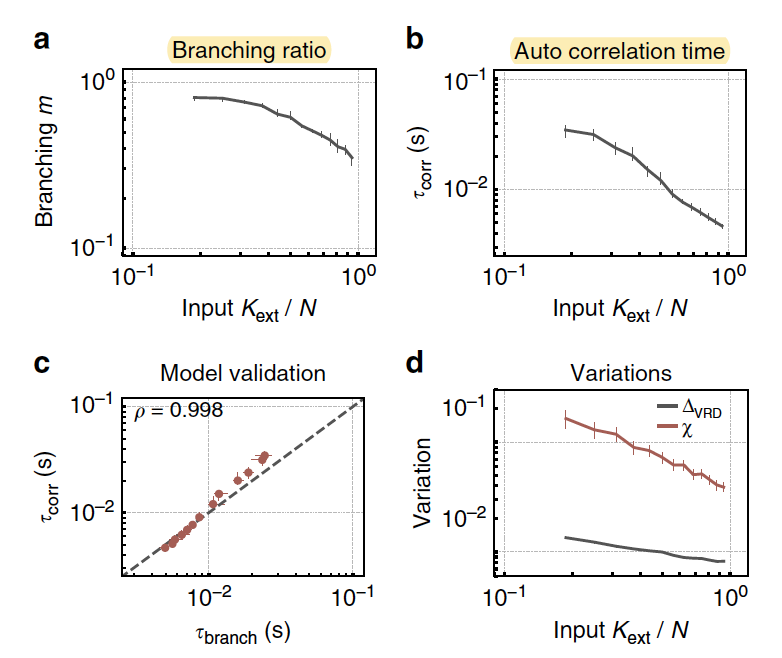
\includegraphics[scale=0.55]{cramer-criticality}
\end{center}

\end{frame}

\begin{frame}[plain]
\frametitle{Balancing internal and recurrent inputs} 



\end{frame}

\begin{frame}[plain]
\frametitle{The role of criticality in information transmission} 

\begin{itemize}
\item What are the synaptic weight distributions before and after optimizing firing rate?
\item Can we generate critical networks by changing 
\end{itemize}


\end{frame}

\begin{frame}[plain]
\frametitle{Higher order correlations} 

Does the correlation structure of the network depend on the correlation structure of the stimulus?

\begin{center}
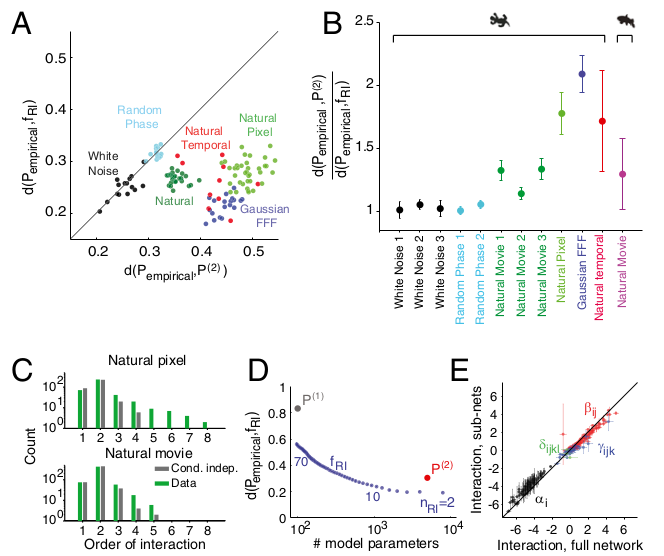
\includegraphics[scale=0.35]{higher-order-interactions}
\end{center}


\end{frame}

\section{Channel coding for neural networks} 

\begin{frame}[plain]
\frametitle{Channel coding for neural networks} 

Networks of neurons can be viewed as a communication channel

Except this communication channel \emph{learns} the transformation $F$ based on the statistical structure of its input $X$. Visual cortex has learned an encoding for visual scenes (that perhaps maximizes information)

\end{frame}


\begin{frame}[plain]
\frametitle{RNN Gradients} 

Say we have a model $\Phi = (W^{0},W^{1})$ and want to use gradient descent to train a network to have a target rate or a target branching parameter. The rate and its associated loss for a single unit is

\begin{equation*}
r(t) = \frac{1}{\Delta t}\int_{t}^{t+\Delta t} d\tau \langle \rho(\tau)\rangle\;\;\;\;\;\mathcal{L} = \alpha(r-r_{0})^{2}
\end{equation*}

We would like the standard update 

\begin{equation*}
\Delta W_{ij} = -\eta \frac{\partial\mathcal{L}}{\partial W_{ij}}
\end{equation*}


But it is intractable to compute $\frac{\partial\mathcal{L}}{\partial W_{ij}}$ since $\rho(t)$ depends on other neurons through space and time.


\end{frame}


\begin{frame}[plain]
\frametitle{Factorizing loss gradients for BPTT} 

BPTT involves unrolling an RNN into a large feedforward network where each layer is a time step. 

\begin{equation*}
\frac{\partial\mathcal{L}}{\partial W^{t}_{ij}} = \frac{\partial\mathcal{L}}{\partial h^{t}_{j}}  \frac{\partial h^{t}_{j}}{{\partial W^{t}_{ij}}} 
\end{equation*}

and the total gradient is a sum over the layers (time)

\begin{equation*}
\frac{\partial\mathcal{L}}{\partial W^{t}_{ij}} = \sum_{t} \frac{\partial\mathcal{L}}{\partial h^{t}_{j}}  \frac{\partial h^{t}_{j}}{{\partial W^{t}_{ij}}} 
\end{equation*}

\end{frame}

\begin{frame}[plain]
\frametitle{Deriving e-prop from BPTT} 

Consider the first term above. The hidden state is computed by some function $h_{j}^{t} = F(z_{j}^{t},h_{j}^{t-1} ,W)$. Backpropagating through time is then

\begin{equation*}
\frac{\partial\mathcal{L}}{\partial h^{t}_{j}} = \frac{\partial\mathcal{L}}{\partial z^{t}_{j}} \frac{\partial z^{t}_{j}}{\partial h^{t}_{j}}  + \frac{\partial\mathcal{L}}{\partial h^{t+1}_{j}} \frac{\partial h^{t+1}_{j}}{\partial h^{t}_{j}} 
\end{equation*}

which must be expressed recursively 

\begin{align*}
\frac{\partial\mathcal{L}}{\partial h^{t}_{j}} &= \frac{\partial\mathcal{L}}{\partial z^{t}_{j}} \frac{\partial z^{t}_{j}}{\partial h^{t}_{j}}  +  \left(\frac{\partial\mathcal{L}}{\partial z^{t+1}_{j}} \frac{\partial z^{t+1}_{j}}{\partial h^{t+1}_{j}}  + (...) \frac{\partial h^{t+2}_{j}}{\partial h^{t+1}_{j}} \right) \frac{\partial h^{t+1}_{j}}{\partial h^{t}_{j}} \\
&= L_{j}^{t} \frac{\partial z^{t}_{j}}{\partial h^{t}_{j}}  +  \left(L_{j}^{t+1} \frac{\partial z^{t+1}_{j}}{\partial h^{t+1}_{j}}  + (...) \frac{\partial h^{t+2}_{j}}{\partial h^{t+1}_{j}} \right) \frac{\partial h^{t+1}_{j}}{\partial h^{t}_{j}}\\
&= L_{j}^{t} \frac{\partial z^{t}_{j}}{\partial h^{t}_{j}}  +  \left(L_{j}^{t+1} \frac{\partial z^{t+1}_{j}}{\partial h^{t+1}_{j}}  + (...) \frac{\partial h^{t+2}_{j}}{\partial h^{t+1}_{j}} \right) \frac{\partial h^{t+1}_{j}}{\partial h^{t}_{j}}
\end{align*}

\end{frame}

\begin{frame}[plain]
\frametitle{Deriving e-prop from BPTT} 

Plugging into the original factorization gives

\begin{equation*}
\frac{\partial\mathcal{L}}{\partial W_{ij}} = \left(\sum_{t}L_{j}^{t} \frac{\partial z^{t}_{j}}{\partial h^{t}_{j}}  +  \left(L_{j}^{t+1} \frac{\partial z^{t+1}_{j}}{\partial h^{t+1}_{j}}  + (...) \frac{\partial h^{t+2}_{j}}{\partial h^{t+1}_{j}} \right) \frac{\partial h^{t+1}_{j}}{\partial h^{t}_{j}} \right)\frac{\partial h^{t'}_{j}}{{\partial W_{ij}}} 
\end{equation*}

You can then collect terms that are multiplied $L_{j}^{t}$

\begin{align*}
\frac{\partial\mathcal{L}}{\partial W_{ij}} &= \sum_{t}L_{j}^{t}\frac{\partial z^{t}_{j}}{\partial h^{t}_{j}} \left( \sum_{t'\leq t} \left(\prod_{t'} \frac{\partial h^{t'+1}_{j}}{\partial h^{t'}_{j}} \right)\frac{\partial h^{t'}_{j}}{{\partial W_{ij}}} \right) \\
&= \sum_{t}L_{j}^{t} \frac{\partial z^{t}_{j}}{\partial h^{t}_{j}}\mathbf{\epsilon_{ij}^{t}} = \sum_{t}L_{j}^{t} e_{ij}^{t} \\
\end{align*}

\end{frame}
\begin{frame}[plain]
\frametitle{Constraining the global firing rate distribution} 

We can define a constraint on the variance of the global firing rate (which simultaneously constrains the mean)

\begin{equation*}
\mathcal{L} = \beta(\sigma- \sigma_{r})^{2}
\;\;\;\;\;\;\; \sigma = \frac{1}{T}\sum_{t} (r - \mu_{r})^{2}
\end{equation*}

where we constrain branching by constraining the variance $s$ of the global firing rate where branching $\rightarrow 1$ as $s \rightarrow 0$.  

\begin{align*}
L_{j}^{t} = \frac{\partial \mathcal{L}}{\partial z_{j}^{t}} = \frac{\partial \mathcal{L}}{\partial \sigma}\frac{\partial \sigma}{\partial n} \frac{\partial n}{\partial z_{j}^{t}}
&= \pm \beta (\sigma- \sigma_{r}) \cdot (r-\mu_{r}) 
\end{align*}

Think push-pull. Some variation is necessary for refractoriness.

\end{frame}


\begin{frame}[plain]
\frametitle{Receptive fields of neurons in a low-rate network} 


\end{frame}

\section{Multivariate information theory} 

\begin{frame}[plain]
\frametitle{Multivariate information theory} 
\end{frame}

\section{Adaptation of the transfer function} 

\begin{frame}[plain]
\frametitle{Adaptation of the transfer function} 
How do neuron transfer functions adapt to stimuli in an unsupervised manner?
\end{frame}

\section{Learning an energy function over phase space} 

\begin{frame}[plain]
\frametitle{Adaptation defines an energy function over phase space} 
\end{frame}

\section{Generalization bounds and density estimation} 

\begin{frame}[plain]
\frametitle{Generalization bounds}
What is the distance of a code defined by a particular energy function $\mathbf{E}$
\end{frame}

\section{The energy function defines a dynamical system} 

\begin{frame}[plain]
\frametitle{The energy function defines a dynamical system} 
\end{frame}


\section{The energy function is a generative model} 

\begin{frame}[plain]
\frametitle{The energy function is a generative model} 
\end{frame}

\section{Application to natural image statistics} 

\begin{frame}[plain]
\frametitle{Application to natural image statistics} 
\end{frame}





\end{document}